Rendered for $t = 150$--$210$\,s (1{,}800 frames, 2{,}052\,s end to end on 4 CPU cores including calibration)
with the corrected parameters; calibration and the trajectory still used the full 11-minute recording.
Fig.~\ref{fig:s24} shows a frame in the right-hand bend at $t=180$\,s, where the first render had put the
ribbon on the verge.

\begin{figure}[H]
\centering
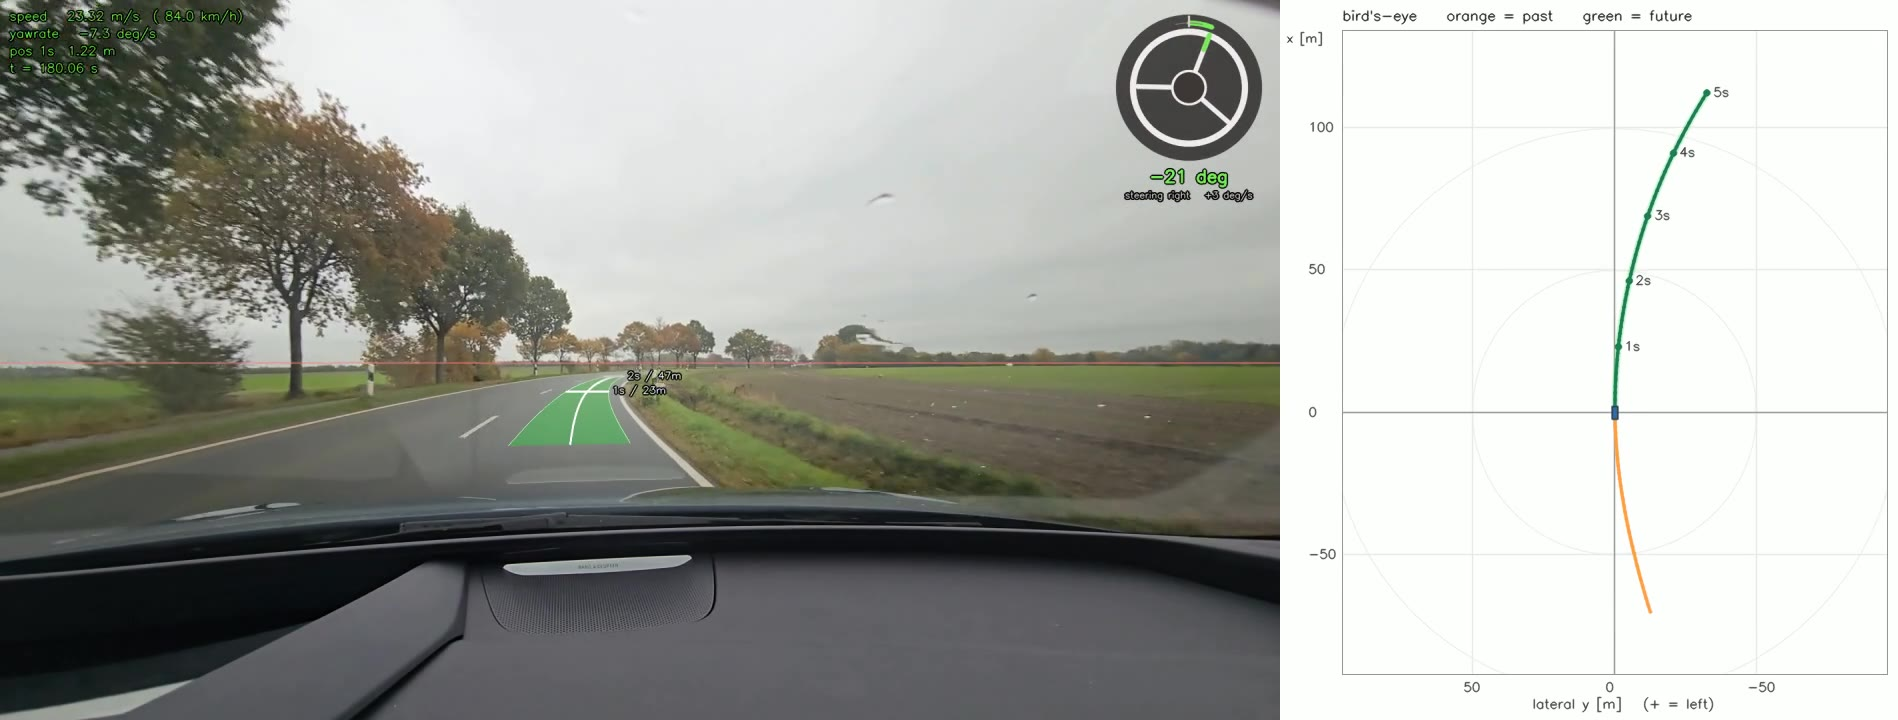
\includegraphics[width=\textwidth]{s24_overlay_30s.jpg}
\caption{S24 Ultra / A6 e-tron, $t = 180.06$\,s, 23.3\,m/s, yaw rate $-7.3^\circ$/s. The future path (green)
stays in the ego lane through the bend; the bird's-eye panel shows the same right turn that the GNSS bearing
confirms (118$^\circ \to$ 151$^\circ$ over 5\,s).}
\label{fig:s24}
\end{figure}

\begin{table}[H]
\centering\small
\begin{tabular}{@{}lc@{}}
\toprule
metric (\texttt{tools/verify\_overlay.py}, every 3rd frame) & value \\
\midrule
frames sampled / straight with both lines / curved or slow & 602 / 29 / 535 \\
path vs lane angle, median (p10, p90) & $-0.14^\circ$ ($-0.96^\circ$, $+0.84^\circ$) \\
offset from lane centre at 10\,m, median & $-0.06$ lane widths \\
offset from lane centre at 25\,m, median & $-0.05$ lane widths \\
ribbon centre inside the lane to 30\,m & 29 / 29 frames \\
ribbon edges (1.923\,m) inside the lane to 30\,m & 26 / 29 frames \\
prediction vs outcome at 20\,m, median (p10, p90) & $+0.01$\,m ($-0.87$, $+0.10$), $n=27$ \\
prediction vs outcome at 30\,m, median (p10, p90) & $+0.01$\,m ($-0.81$, $+0.14$), $n=24$ \\
\bottomrule
\end{tabular}
\caption{Corrected render, \meas{} (\texttt{verify\_fix.json}). The window is mostly bends, so only 29 frames
qualify as straight with two visible lines; the numbers are encouraging but a small sample, and the
$-0.8$\,m tail of prediction vs outcome is not yet explained. The full-length render and a check over all
11 minutes are the next step.}
\end{table}
